% The two curation activities and the selection between them.
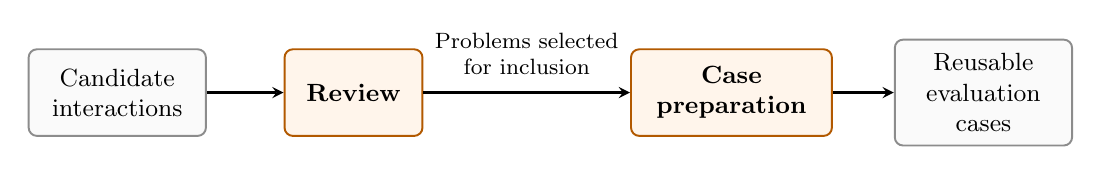
\begin{tikzpicture}[
  activity/.style={
    draw=orange!70!black, fill=orange!8,
    rounded corners=3pt, line width=0.7pt,
    minimum height=1.1cm, inner sep=5pt,
    align=center, font=\small\bfseries
  },
  artifact/.style={
    draw=black!45, fill=black!2,
    rounded corners=3pt, line width=0.7pt,
    text width=1.9cm, minimum height=1.1cm, inner sep=5pt,
    align=center, font=\small
  },
  flow/.style={->, >=stealth, line width=0.8pt},
  transition/.style={align=center, font=\footnotesize, inner sep=2pt}
]
  \node[artifact] (candidates) at (0,0) {Candidate\\interactions};
  \node[activity, text width=1.4cm] (review) at (3,0) {Review};
  \node[activity, text width=2.2cm] (preparation) at (7.8,0)
    {Case\\preparation};
  \node[artifact] (cases) at (11,0) {Reusable\\evaluation\\cases};

  \draw[flow] (candidates.east) -- (review.west);
  \draw[flow] (review.east) -- node[transition, above=4pt]
    {Problems selected\\for inclusion} (preparation.west);
  \draw[flow] (preparation.east) -- (cases.west);
\end{tikzpicture}
